\section{Metodología utilizada}
\label{sec:Methodology}

Con la Programación orientada a Aspectos, desarrollamos dos conceptos \ldots el
de Obervabilidad y el de Transaccionalidad.

\subsection{ Observabilidad}
	El aspecto Observable tiene como objetivos:
	\begin{itemize}
	
	  \item Convertir los objetos de dominio en observable, sin que el cliente los
	  modifique.
	  
	  \item Tirar eventos cuando se modifica un atributo, 
	\end{itemize}

\subsubsection{Aspecto Transaccional:} 

	{\bf Objetivos:}
	\begin{itemize}

	  \item Permitir deshacer los cambios. (rollback).

	  \item Permitir el trabajo concurrente (nivel de aislamiento)
	  
	  \item Que utilice a los objetos en forma transparente.
	  
	  \item Mantener la identidad del objeto.
	  
	  \item Soportar transacciones anidadas.
	   
	\end{itemize} 
	
	Interfaz que nos provee las transacciones:
	\begin{itemize}
	  \item {\bf beginTransaction}  \emph{empezar una transacción}
	  \item {\bf commit} \emph{impactar los cambios realizados en esa transacción}
	  \item {\bf rollback} \emph{revertir los cambios realizados en esa
	  transacción}
	\end{itemize}


	{\bf Uso}
	\begin{itemize}
	  \item Todo el trabajo se realiza dentro de un contexto transaccional.
	  
	  \item Las modificaciones de los objetos solo pueden ser vistos dento del
	  mismo contexto, si todavía no se hizo el commit.
	   
	  \item El objeto no se modifica, hasta que no se confirme la transacción.
	  
	   \item El contexto transaccional esta asociado a thread actual.
	\end{itemize}


	{\bf Modelo Transaccional}
	
	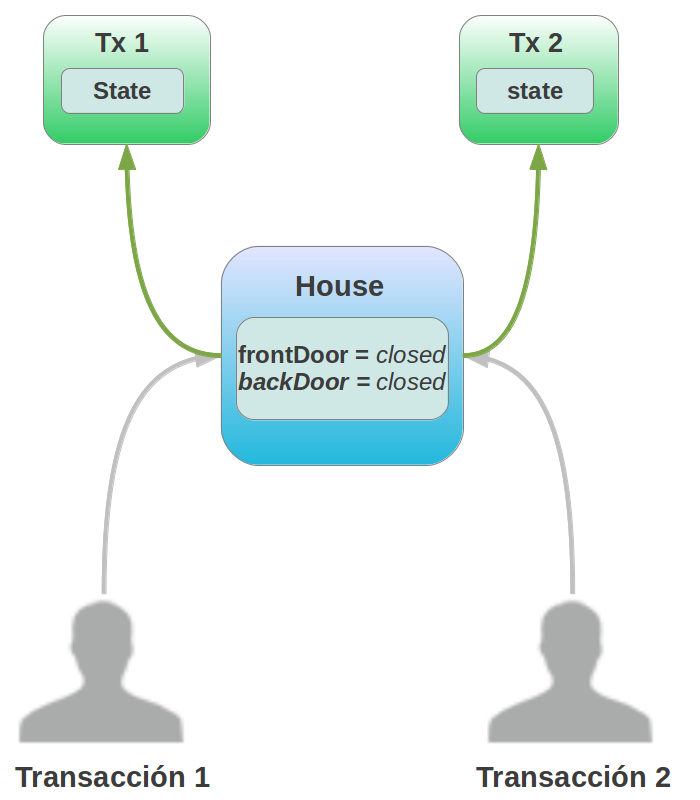
\includegraphics[width=350px, height=300px]{img/transacionalModel}
	
	{\bf Caso de uso}
	
	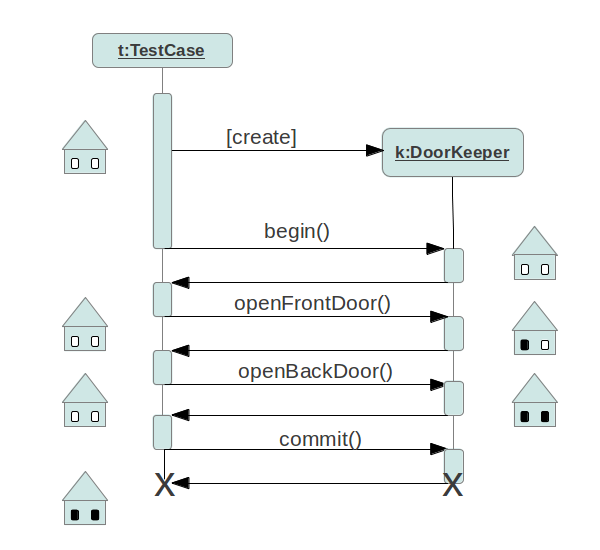
\includegraphics[width=400px, height=300px]{img/tescasePOT}
	
	{\bf Contexto de transacciones anidadas (1/8)}\\
	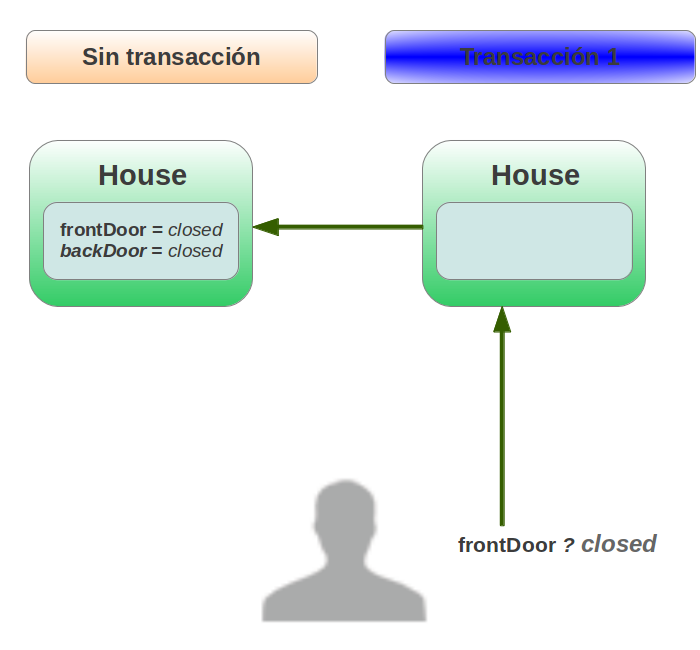
\includegraphics[width=400px, height=300px]{img/contextoAninado1}
	
	{\bf Contexto de transacciones anidadas (2/8)}\\
	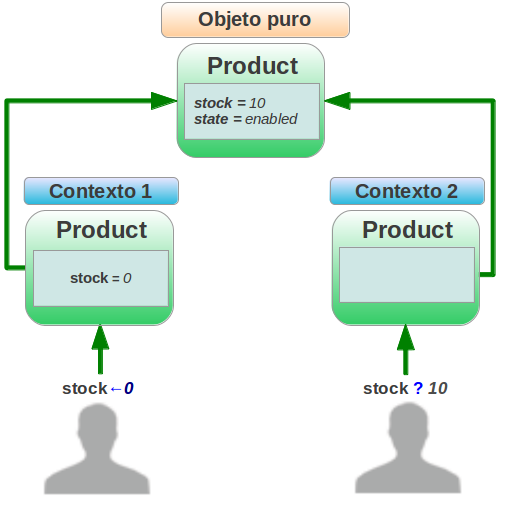
\includegraphics[width=400px, height=300px]{img/contextoAninado2}
	
	{\bf Contexto de transacciones anidadas (3/8)}\\
	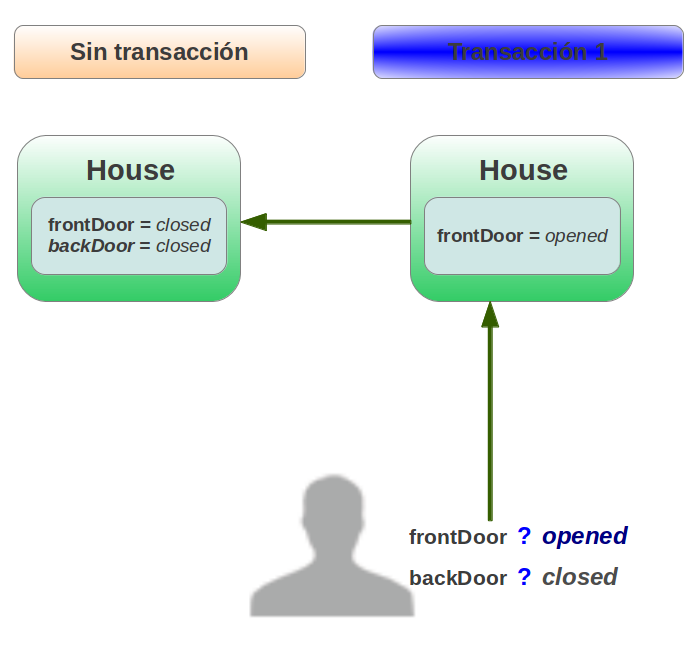
\includegraphics[width=400px, height=300px]{img/contextoAninado3}
	
	{\bf Contexto de transacciones anidadas (4/8)}\\
	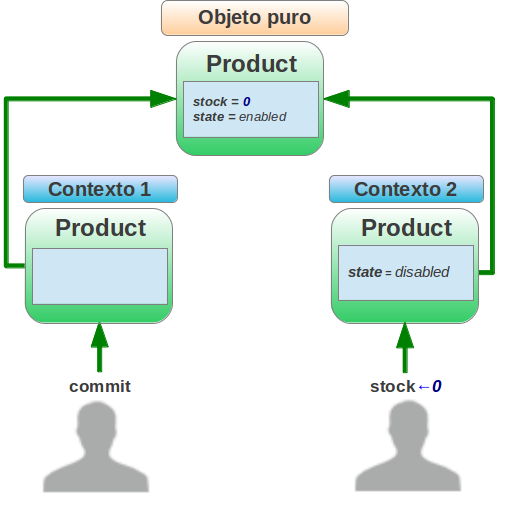
\includegraphics[width=400px, height=300px]{img/contextoAninado4}
	
	{\bf Contexto de transacciones anidadas (5/8)}\\
	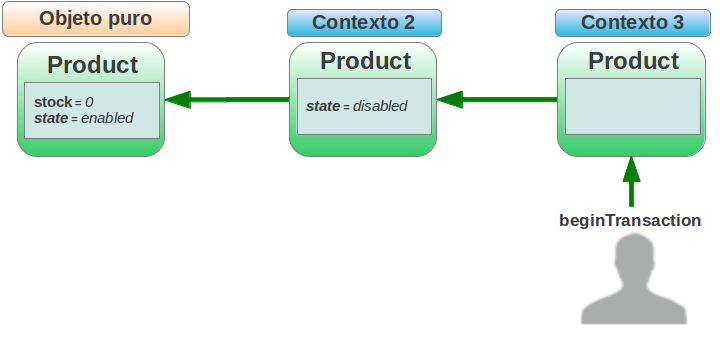
\includegraphics[width=400px, height=300px]{img/contextoAninado5}

	{\bf Contexto de transacciones anidadas (6/8)}\\
	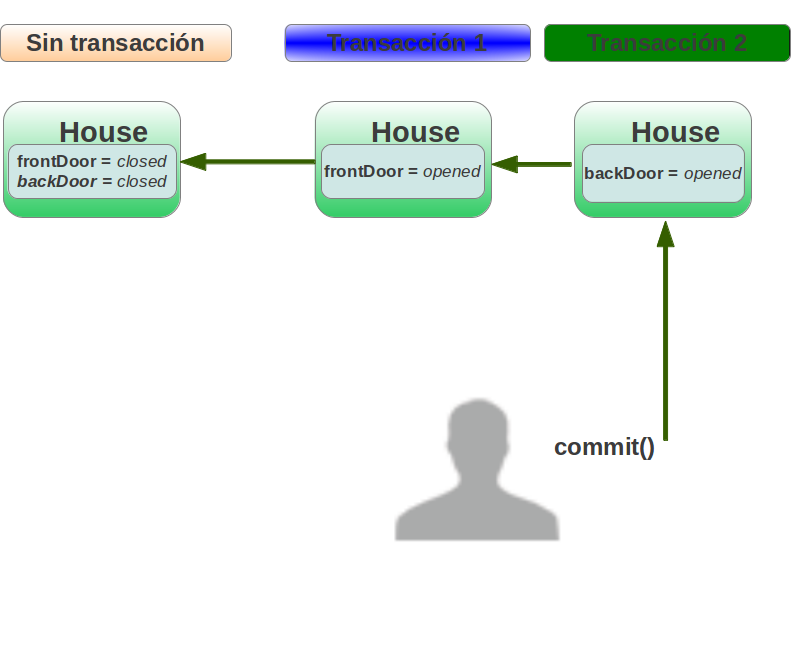
\includegraphics[width=400px, height=300px]{img/contextoAninado6}

	{\bf Contexto de transacciones anidadas (7/8)}\\
	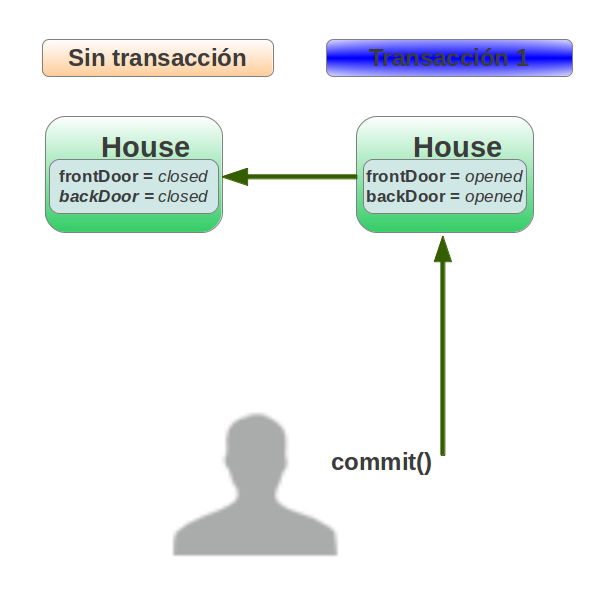
\includegraphics[width=350px, height=300px]{img/contextoAninado7}

	{\bf Contexto de transacciones anidadas (8/8)}\\
	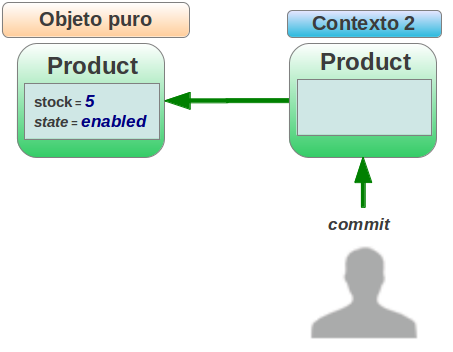
\includegraphics[width=150px, height=150px]{img/contextoAninado8}
	
\subsubsection{Unión de los Aspectos:}
No se como contarlo acá, sin decir que esta con el arena. 
	


Primero contás sobre eventos, luegos sobre transacciones y finalmente la unión.
